% This file was created by matlab2tikz.
%
%The latest updates can be retrieved from
%  http://www.mathworks.com/matlabcentral/fileexchange/22022-matlab2tikz-matlab2tikz
%where you can also make suggestions and rate matlab2tikz.
%
\definecolor{mycolor1}{rgb}{0.00000,0.44700,0.74100}%
\definecolor{mycolor2}{rgb}{0.00000,0.44706,0.74118}%
\definecolor{mycolor3}{rgb}{0.85098,0.32549,0.09804}%
\definecolor{mycolor4}{rgb}{0.49400,0.18400,0.55600}%
\definecolor{mycolor5}{rgb}{0.46667,0.67451,0.18824}%
%
\makeatletter
\newcommand\resetstackedplots{
    \makeatletter
    \pgfplots@stacked@isfirstplottrue
    \makeatother
    \addplot [forget plot,draw=none] coordinates{(1,0) (5,0) (10,0) (15,0) (20,0)};
}
\makeatother
%
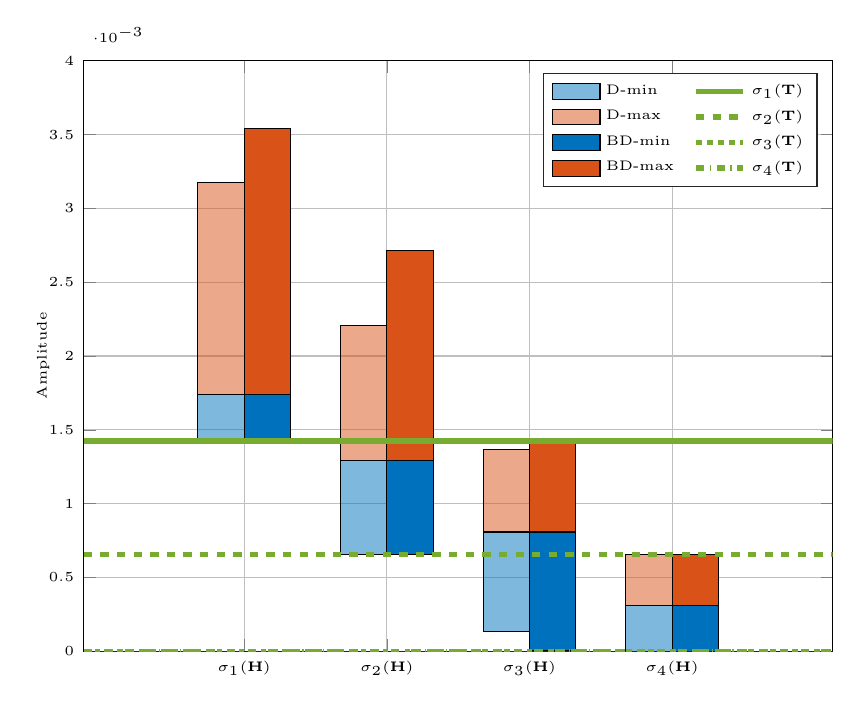
\begin{tikzpicture}

\begin{axis}[%
width=9.509cm,
height=7.5cm,
at={(0cm,0cm)},
scale only axis,
bar width=0.325,
xmin=-0.125,
xmax=5.125,
xtick={1,2,3,4},
xticklabels={{$\sigma_1(\mathbf{H})$},{$\sigma_2(\mathbf{H})$},{$\sigma_3(\mathbf{H})$},{$\sigma_4(\mathbf{H})$}},
ymin=0,
ymax=0.004,
% ylabel style={font=\color{white!15!black}},
ylabel={Amplitude},
axis background/.style={fill=white},
xmajorgrids,
ymajorgrids,
legend style={legend cell align=left, align=left, draw=white!15!black},
legend columns=4,
transpose legend,
legend style={/tikz/column 2/.style={column sep=5pt}},
font=\tiny,
title style={font=\tiny},
label style={font=\tiny},
ticklabel style={font=\tiny},
legend style={font=\tiny},
y label style={yshift=-7pt}
]
\addplot[ybar stacked, fill=none, draw=none, forget plot] table[row sep=crcr] {%
0.8375	0.00142543267002251\\
1.8375	0.000656306214245826\\
2.8375	0.000132970460937413\\
3.8375	3.2994096547908e-20\\
};
\addplot[forget plot, color=white!15!black] table[row sep=crcr] {%
-0.125	0\\
5.125	0\\
};
\addplot[ybar stacked, fill=mycolor2, fill opacity=0.5, draw=black, area legend] table[row sep=crcr] {%
0.8375	0.000316188517375316\\
1.8375	0.000636356951614819\\
2.8375	0.000675093172956787\\
3.8375	0.000311028141103694\\
};
\addplot[forget plot, color=white!15!black] table[row sep=crcr] {%
-0.125	0\\
5.125	0\\
};
\addlegendentry{D-min}

\addplot[ybar stacked, fill=mycolor3, fill opacity=0.5, draw=black, area legend] table[row sep=crcr] {%
0.8375	0.00143103448582135\\
1.8375	0.000911508088276409\\
2.8375	0.000557699498413843\\
3.8375	0.000345278073129164\\
};
\addplot[forget plot, color=white!15!black] table[row sep=crcr] {%
-0.125	0\\
5.125	0\\
};
\addlegendentry{D-max}

\resetstackedplots

\addplot[ybar stacked, fill=none, draw=none, forget plot] table[row sep=crcr] {%
1.1625	0.00142543579700608\\
2.1625	0.00065631304524136\\
3.1625	5.27477395632166e-06\\
4.1625	4.21048388214027e-08\\
};
\addplot[forget plot, color=white!15!black] table[row sep=crcr] {%
-0.125	0\\
5.125	0\\
};
\addplot[ybar stacked, fill=mycolor2, draw=black, area legend] table[row sep=crcr] {%
1.1625	0.000316185390391755\\
2.1625	0.000636350120619285\\
3.1625	0.000802788859937878\\
4.1625	0.000310986036264873\\
};
\addplot[forget plot, color=white!15!black] table[row sep=crcr] {%
-0.125	0\\
5.125	0\\
};
\addlegendentry{BD-min}

\addplot[ybar stacked, fill=mycolor3, draw=black, area legend] table[row sep=crcr] {%
1.1625	0.00179647322615157\\
2.1625	0.00141980780340078\\
3.1625	0.000617369035963568\\
4.1625	0.000345278072973618\\
};
\addplot[forget plot, color=white!15!black] table[row sep=crcr] {%
-0.125	0\\
5.125	0\\
};
\addlegendentry{BD-max}

\addplot [color=mycolor5, line width=2.0pt]
  table[row sep=crcr]{%
-0.125	0.00142543266997377\\
5.125	0.00142543266997377\\
};
\addlegendentry{$\sigma_1(\mathbf{T})$}

\addplot [color=mycolor5, dashed, line width=2.0pt]
  table[row sep=crcr]{%
-0.125	0.000656306214237067\\
5.125	0.000656306214237067\\
};
\addlegendentry{$\sigma_2(\mathbf{T})$}

\addplot [color=mycolor5, dotted, line width=2.0pt]
  table[row sep=crcr]{%
-0.125	1.83134593569563e-11\\
5.125	1.83134593569563e-11\\
};
\addlegendentry{$\sigma_3(\mathbf{T})$}

\addplot [color=mycolor5, dashdotted, line width=2.0pt]
  table[row sep=crcr]{%
-0.125	8.07634856586464e-12\\
5.125	8.07634856586464e-12\\
};
\addlegendentry{$\sigma_4(\mathbf{T})$}

\end{axis}
\end{tikzpicture}%
